% !TEX encoding = UTF-8 Unicode
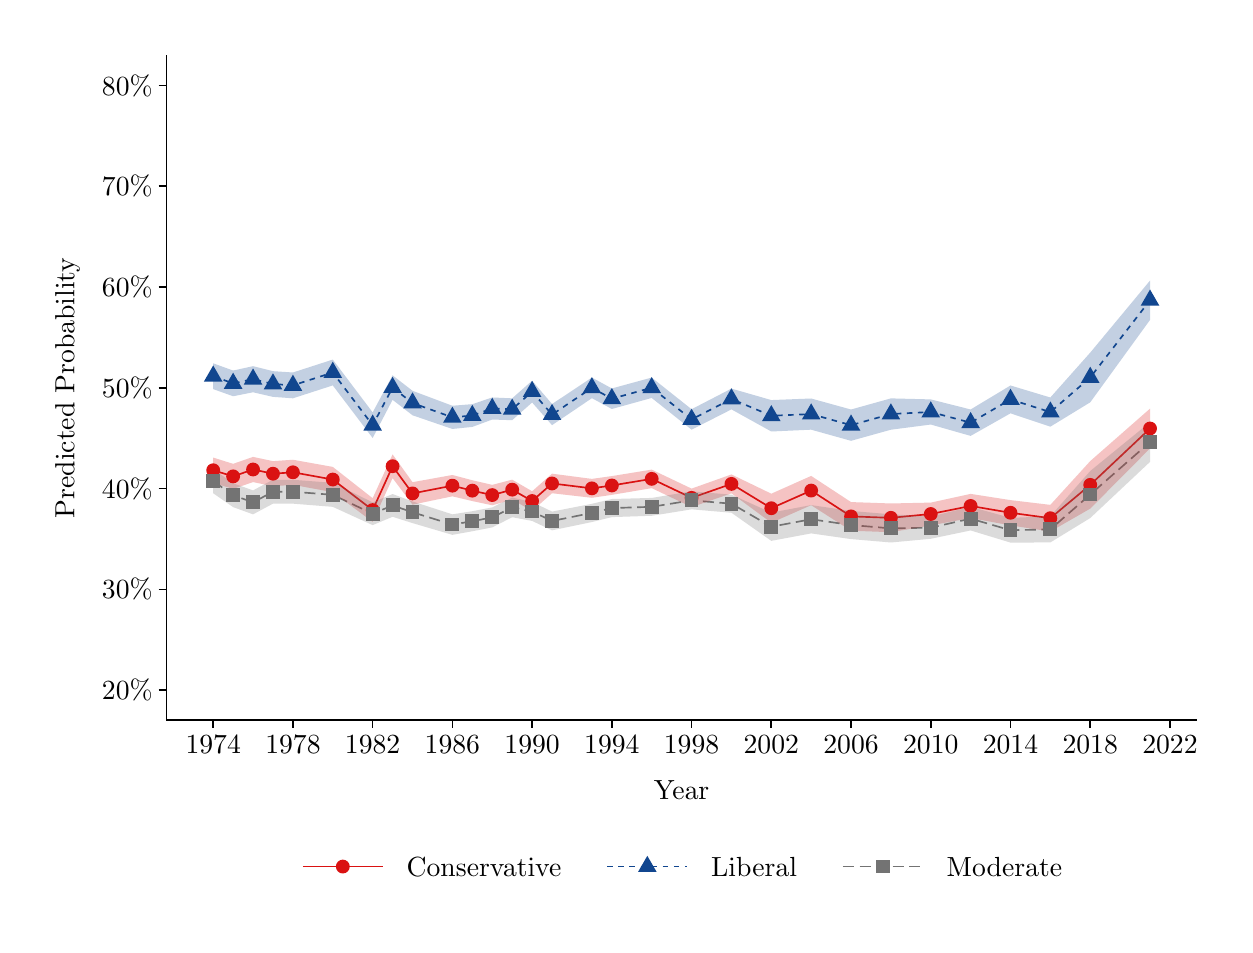
\begin{tikzpicture}[x=1pt,y=1pt]
\definecolor{fillColor}{RGB}{255,255,255}
\path[use as bounding box,fill=fillColor,fill opacity=0.00] (0,0) rectangle (432.48,324.36);
\begin{scope}
\path[clip] (  0.00,  0.00) rectangle (432.48,324.36);
\definecolor{fillColor}{RGB}{255,255,255}

\path[fill=fillColor] ( -0.00,  0.00) rectangle (432.48,324.36);
\end{scope}
\begin{scope}
\path[clip] ( 50.11, 74.07) rectangle (422.48,314.36);
\definecolor{fillColor}{RGB}{255,255,255}

\path[fill=fillColor] ( 50.11, 74.07) rectangle (422.48,314.36);
\definecolor{drawColor}{RGB}{218,18,18}

\path[draw=drawColor,line width= 0.6pt,line join=round] ( 67.04,164.43) --
	( 74.24,162.22) --
	( 81.44,164.71) --
	( 88.64,163.18) --
	( 95.85,163.69) --
	(110.25,161.08) --
	(124.66,150.05) --
	(131.86,165.89) --
	(139.06,156.06) --
	(153.47,158.86) --
	(160.67,157.06) --
	(167.87,155.46) --
	(175.07,157.42) --
	(182.28,153.31) --
	(189.48,159.66) --
	(203.88,157.89) --
	(211.09,158.93) --
	(225.49,161.32) --
	(239.90,154.46) --
	(254.30,159.50) --
	(268.71,150.71) --
	(283.11,157.09) --
	(297.52,147.76) --
	(311.92,147.24) --
	(326.33,148.62) --
	(340.73,151.53) --
	(355.14,149.07) --
	(369.54,147.11) --
	(383.95,159.15) --
	(405.56,179.52);
\definecolor{drawColor}{RGB}{17,70,143}

\path[draw=drawColor,line width= 0.6pt,dash pattern=on 2pt off 2pt ,line join=round] ( 67.04,198.41) --
	( 74.24,195.82) --
	( 81.44,197.33) --
	( 88.64,195.59) --
	( 95.85,195.10) --
	(110.25,199.76) --
	(124.66,180.71) --
	(131.86,194.31) --
	(139.06,188.72) --
	(153.47,183.55) --
	(160.67,184.20) --
	(167.87,186.75) --
	(175.07,186.47) --
	(182.28,192.86) --
	(189.48,184.54) --
	(203.88,194.20) --
	(211.09,190.28) --
	(225.49,194.24) --
	(239.90,182.79) --
	(254.30,190.19) --
	(268.71,184.12) --
	(283.11,184.73) --
	(297.52,180.72) --
	(311.92,184.74) --
	(326.33,185.49) --
	(340.73,181.62) --
	(355.14,190.03) --
	(369.54,185.45) --
	(383.95,197.95) --
	(405.56,225.87);
\definecolor{drawColor}{gray}{0.45}

\path[draw=drawColor,line width= 0.6pt,dash pattern=on 4pt off 2pt ,line join=round] ( 67.04,160.49) --
	( 74.24,155.42) --
	( 81.44,152.82) --
	( 88.64,156.68) --
	( 95.85,156.67) --
	(110.25,155.55) --
	(124.66,148.71) --
	(131.86,151.73) --
	(139.06,149.25) --
	(153.47,144.80) --
	(160.67,146.01) --
	(167.87,147.39) --
	(175.07,151.01) --
	(182.28,149.54) --
	(189.48,146.10) --
	(203.88,149.01) --
	(211.09,150.77) --
	(225.49,151.21) --
	(239.90,153.56) --
	(254.30,152.35) --
	(268.71,144.02) --
	(283.11,146.73) --
	(297.52,144.64) --
	(311.92,143.43) --
	(326.33,143.68) --
	(340.73,146.95) --
	(355.14,142.76) --
	(369.54,143.07) --
	(383.95,155.66) --
	(405.56,174.63);
\definecolor{fillColor}{RGB}{218,18,18}

\path[fill=fillColor,fill opacity=0.25] ( 67.04,169.01) --
	( 74.24,166.75) --
	( 81.44,169.26) --
	( 88.64,167.72) --
	( 95.85,168.23) --
	(110.25,165.64) --
	(124.66,154.33) --
	(131.86,170.16) --
	(139.06,160.12) --
	(153.47,162.72) --
	(160.67,160.82) --
	(167.87,159.15) --
	(175.07,161.03) --
	(182.28,156.84) --
	(189.48,163.19) --
	(203.88,161.31) --
	(211.09,162.32) --
	(225.49,164.66) --
	(239.90,157.80) --
	(254.30,162.92) --
	(268.71,155.96) --
	(283.11,162.38) --
	(297.52,152.93) --
	(311.92,152.43) --
	(326.33,152.74) --
	(340.73,155.89) --
	(355.14,153.64) --
	(369.54,151.92) --
	(383.95,167.74) --
	(405.56,186.70) --
	(405.56,172.33) --
	(383.95,150.56) --
	(369.54,142.30) --
	(355.14,144.50) --
	(340.73,147.18) --
	(326.33,144.49) --
	(311.92,142.05) --
	(297.52,142.58) --
	(283.11,151.80) --
	(268.71,145.46) --
	(254.30,156.09) --
	(239.90,151.12) --
	(225.49,157.97) --
	(211.09,155.54) --
	(203.88,154.48) --
	(189.48,156.13) --
	(182.28,149.77) --
	(175.07,153.82) --
	(167.87,151.77) --
	(160.67,153.30) --
	(153.47,155.01) --
	(139.06,152.00) --
	(131.86,161.61) --
	(124.66,145.78) --
	(110.25,156.53) --
	( 95.85,159.16) --
	( 88.64,158.65) --
	( 81.44,160.16) --
	( 74.24,157.68) --
	( 67.04,159.84) --
	cycle;

\path[] ( 67.04,169.01) --
	( 74.24,166.75) --
	( 81.44,169.26) --
	( 88.64,167.72) --
	( 95.85,168.23) --
	(110.25,165.64) --
	(124.66,154.33) --
	(131.86,170.16) --
	(139.06,160.12) --
	(153.47,162.72) --
	(160.67,160.82) --
	(167.87,159.15) --
	(175.07,161.03) --
	(182.28,156.84) --
	(189.48,163.19) --
	(203.88,161.31) --
	(211.09,162.32) --
	(225.49,164.66) --
	(239.90,157.80) --
	(254.30,162.92) --
	(268.71,155.96) --
	(283.11,162.38) --
	(297.52,152.93) --
	(311.92,152.43) --
	(326.33,152.74) --
	(340.73,155.89) --
	(355.14,153.64) --
	(369.54,151.92) --
	(383.95,167.74) --
	(405.56,186.70);

\path[] (405.56,172.33) --
	(383.95,150.56) --
	(369.54,142.30) --
	(355.14,144.50) --
	(340.73,147.18) --
	(326.33,144.49) --
	(311.92,142.05) --
	(297.52,142.58) --
	(283.11,151.80) --
	(268.71,145.46) --
	(254.30,156.09) --
	(239.90,151.12) --
	(225.49,157.97) --
	(211.09,155.54) --
	(203.88,154.48) --
	(189.48,156.13) --
	(182.28,149.77) --
	(175.07,153.82) --
	(167.87,151.77) --
	(160.67,153.30) --
	(153.47,155.01) --
	(139.06,152.00) --
	(131.86,161.61) --
	(124.66,145.78) --
	(110.25,156.53) --
	( 95.85,159.16) --
	( 88.64,158.65) --
	( 81.44,160.16) --
	( 74.24,157.68) --
	( 67.04,159.84);
\definecolor{fillColor}{RGB}{17,70,143}

\path[fill=fillColor,fill opacity=0.25] ( 67.04,203.07) --
	( 74.24,200.46) --
	( 81.44,202.04) --
	( 88.64,200.23) --
	( 95.85,199.76) --
	(110.25,204.42) --
	(124.66,185.34) --
	(131.86,198.73) --
	(139.06,193.14) --
	(153.47,187.74) --
	(160.67,188.31) --
	(167.87,190.73) --
	(175.07,190.42) --
	(182.28,196.80) --
	(189.48,188.36) --
	(203.88,197.93) --
	(211.09,193.99) --
	(225.49,197.92) --
	(239.90,186.48) --
	(254.30,193.94) --
	(268.71,189.79) --
	(283.11,190.36) --
	(297.52,186.38) --
	(311.92,190.40) --
	(326.33,190.03) --
	(340.73,186.39) --
	(355.14,195.06) --
	(369.54,190.72) --
	(383.95,206.93) --
	(405.56,232.97) --
	(405.56,218.76) --
	(383.95,188.98) --
	(369.54,180.18) --
	(355.14,185.00) --
	(340.73,176.85) --
	(326.33,180.95) --
	(311.92,179.08) --
	(297.52,175.07) --
	(283.11,179.09) --
	(268.71,178.44) --
	(254.30,186.43) --
	(239.90,179.10) --
	(225.49,190.56) --
	(211.09,186.57) --
	(203.88,190.48) --
	(189.48,180.73) --
	(182.28,188.92) --
	(175.07,182.52) --
	(167.87,182.76) --
	(160.67,180.09) --
	(153.47,179.35) --
	(139.06,184.30) --
	(131.86,189.89) --
	(124.66,176.08) --
	(110.25,195.09) --
	( 95.85,190.43) --
	( 88.64,190.95) --
	( 81.44,192.61) --
	( 74.24,191.18) --
	( 67.04,193.75) --
	cycle;

\path[] ( 67.04,203.07) --
	( 74.24,200.46) --
	( 81.44,202.04) --
	( 88.64,200.23) --
	( 95.85,199.76) --
	(110.25,204.42) --
	(124.66,185.34) --
	(131.86,198.73) --
	(139.06,193.14) --
	(153.47,187.74) --
	(160.67,188.31) --
	(167.87,190.73) --
	(175.07,190.42) --
	(182.28,196.80) --
	(189.48,188.36) --
	(203.88,197.93) --
	(211.09,193.99) --
	(225.49,197.92) --
	(239.90,186.48) --
	(254.30,193.94) --
	(268.71,189.79) --
	(283.11,190.36) --
	(297.52,186.38) --
	(311.92,190.40) --
	(326.33,190.03) --
	(340.73,186.39) --
	(355.14,195.06) --
	(369.54,190.72) --
	(383.95,206.93) --
	(405.56,232.97);

\path[] (405.56,218.76) --
	(383.95,188.98) --
	(369.54,180.18) --
	(355.14,185.00) --
	(340.73,176.85) --
	(326.33,180.95) --
	(311.92,179.08) --
	(297.52,175.07) --
	(283.11,179.09) --
	(268.71,178.44) --
	(254.30,186.43) --
	(239.90,179.10) --
	(225.49,190.56) --
	(211.09,186.57) --
	(203.88,190.48) --
	(189.48,180.73) --
	(182.28,188.92) --
	(175.07,182.52) --
	(167.87,182.76) --
	(160.67,180.09) --
	(153.47,179.35) --
	(139.06,184.30) --
	(131.86,189.89) --
	(124.66,176.08) --
	(110.25,195.09) --
	( 95.85,190.43) --
	( 88.64,190.95) --
	( 81.44,192.61) --
	( 74.24,191.18) --
	( 67.04,193.75);
\definecolor{fillColor}{RGB}{115,115,115}

\path[fill=fillColor,fill opacity=0.25] ( 67.04,164.85) --
	( 74.24,159.73) --
	( 81.44,157.15) --
	( 88.64,161.00) --
	( 95.85,160.98) --
	(110.25,159.89) --
	(124.66,152.82) --
	(131.86,155.84) --
	(139.06,153.16) --
	(153.47,148.50) --
	(160.67,149.63) --
	(167.87,151.01) --
	(175.07,154.55) --
	(182.28,152.96) --
	(189.48,149.49) --
	(203.88,152.30) --
	(211.09,154.04) --
	(225.49,154.43) --
	(239.90,156.81) --
	(254.30,155.61) --
	(268.71,149.12) --
	(283.11,151.84) --
	(297.52,149.72) --
	(311.92,148.52) --
	(326.33,147.69) --
	(340.73,151.22) --
	(355.14,147.23) --
	(369.54,147.79) --
	(383.95,164.16) --
	(405.56,181.80) --
	(405.56,167.47) --
	(383.95,147.16) --
	(369.54,138.35) --
	(355.14,138.29) --
	(340.73,142.68) --
	(326.33,139.67) --
	(311.92,138.33) --
	(297.52,139.56) --
	(283.11,141.61) --
	(268.71,138.92) --
	(254.30,149.08) --
	(239.90,150.31) --
	(225.49,147.98) --
	(211.09,147.50) --
	(203.88,145.72) --
	(189.48,142.72) --
	(182.28,146.12) --
	(175.07,147.47) --
	(167.87,143.78) --
	(160.67,142.39) --
	(153.47,141.09) --
	(139.06,145.34) --
	(131.86,147.62) --
	(124.66,144.61) --
	(110.25,151.21) --
	( 95.85,152.36) --
	( 88.64,152.36) --
	( 81.44,148.50) --
	( 74.24,151.11) --
	( 67.04,156.12) --
	cycle;

\path[] ( 67.04,164.85) --
	( 74.24,159.73) --
	( 81.44,157.15) --
	( 88.64,161.00) --
	( 95.85,160.98) --
	(110.25,159.89) --
	(124.66,152.82) --
	(131.86,155.84) --
	(139.06,153.16) --
	(153.47,148.50) --
	(160.67,149.63) --
	(167.87,151.01) --
	(175.07,154.55) --
	(182.28,152.96) --
	(189.48,149.49) --
	(203.88,152.30) --
	(211.09,154.04) --
	(225.49,154.43) --
	(239.90,156.81) --
	(254.30,155.61) --
	(268.71,149.12) --
	(283.11,151.84) --
	(297.52,149.72) --
	(311.92,148.52) --
	(326.33,147.69) --
	(340.73,151.22) --
	(355.14,147.23) --
	(369.54,147.79) --
	(383.95,164.16) --
	(405.56,181.80);

\path[] (405.56,167.47) --
	(383.95,147.16) --
	(369.54,138.35) --
	(355.14,138.29) --
	(340.73,142.68) --
	(326.33,139.67) --
	(311.92,138.33) --
	(297.52,139.56) --
	(283.11,141.61) --
	(268.71,138.92) --
	(254.30,149.08) --
	(239.90,150.31) --
	(225.49,147.98) --
	(211.09,147.50) --
	(203.88,145.72) --
	(189.48,142.72) --
	(182.28,146.12) --
	(175.07,147.47) --
	(167.87,143.78) --
	(160.67,142.39) --
	(153.47,141.09) --
	(139.06,145.34) --
	(131.86,147.62) --
	(124.66,144.61) --
	(110.25,151.21) --
	( 95.85,152.36) --
	( 88.64,152.36) --
	( 81.44,148.50) --
	( 74.24,151.11) --
	( 67.04,156.12);
\definecolor{fillColor}{RGB}{17,70,143}

\path[fill=fillColor] ( 67.04,202.30) --
	( 70.40,196.47) --
	( 63.67,196.47) --
	cycle;

\path[fill=fillColor] ( 74.24,199.70) --
	( 77.60,193.88) --
	( 70.87,193.88) --
	cycle;

\path[fill=fillColor] ( 81.44,201.21) --
	( 84.80,195.38) --
	( 78.08,195.38) --
	cycle;

\path[fill=fillColor] ( 88.64,199.47) --
	( 92.01,193.65) --
	( 85.28,193.65) --
	cycle;

\path[fill=fillColor] ( 95.85,198.98) --
	( 99.21,193.15) --
	( 92.48,193.15) --
	cycle;

\path[fill=fillColor] (110.25,203.64) --
	(113.62,197.81) --
	(106.89,197.81) --
	cycle;

\path[fill=fillColor] (124.66,184.59) --
	(128.02,178.77) --
	(121.29,178.77) --
	cycle;

\path[fill=fillColor] (131.86,198.19) --
	(135.22,192.37) --
	(128.50,192.37) --
	cycle;

\path[fill=fillColor] (139.06,192.60) --
	(142.43,186.78) --
	(135.70,186.78) --
	cycle;

\path[fill=fillColor] (153.47,187.43) --
	(156.83,181.61) --
	(150.10,181.61) --
	cycle;

\path[fill=fillColor] (160.67,188.09) --
	(164.03,182.26) --
	(157.31,182.26) --
	cycle;

\path[fill=fillColor] (167.87,190.63) --
	(171.24,184.80) --
	(164.51,184.80) --
	cycle;

\path[fill=fillColor] (175.07,190.35) --
	(178.44,184.53) --
	(171.71,184.53) --
	cycle;

\path[fill=fillColor] (182.28,196.74) --
	(185.64,190.92) --
	(178.91,190.92) --
	cycle;

\path[fill=fillColor] (189.48,188.43) --
	(192.84,182.60) --
	(186.12,182.60) --
	cycle;

\path[fill=fillColor] (203.88,198.09) --
	(207.25,192.26) --
	(200.52,192.26) --
	cycle;

\path[fill=fillColor] (211.09,194.16) --
	(214.45,188.34) --
	(207.72,188.34) --
	cycle;

\path[fill=fillColor] (225.49,198.12) --
	(228.86,192.30) --
	(222.13,192.30) --
	cycle;

\path[fill=fillColor] (239.90,186.68) --
	(243.26,180.85) --
	(236.53,180.85) --
	cycle;

\path[fill=fillColor] (254.30,194.07) --
	(257.67,188.24) --
	(250.94,188.24) --
	cycle;

\path[fill=fillColor] (268.71,188.00) --
	(272.07,182.17) --
	(265.34,182.17) --
	cycle;

\path[fill=fillColor] (283.11,188.61) --
	(286.48,182.79) --
	(279.75,182.79) --
	cycle;

\path[fill=fillColor] (297.52,184.61) --
	(300.88,178.78) --
	(294.15,178.78) --
	cycle;

\path[fill=fillColor] (311.92,188.62) --
	(315.29,182.80) --
	(308.56,182.80) --
	cycle;

\path[fill=fillColor] (326.33,189.37) --
	(329.69,183.55) --
	(322.96,183.55) --
	cycle;

\path[fill=fillColor] (340.73,185.50) --
	(344.10,179.68) --
	(337.37,179.68) --
	cycle;

\path[fill=fillColor] (355.14,193.92) --
	(358.50,188.09) --
	(351.77,188.09) --
	cycle;

\path[fill=fillColor] (369.54,189.33) --
	(372.91,183.50) --
	(366.18,183.50) --
	cycle;

\path[fill=fillColor] (383.95,201.84) --
	(387.31,196.01) --
	(380.58,196.01) --
	cycle;

\path[fill=fillColor] (405.56,229.75) --
	(408.92,223.92) --
	(402.19,223.92) --
	cycle;
\definecolor{fillColor}{RGB}{218,18,18}

\path[fill=fillColor] ( 67.04,164.43) circle (  2.50);

\path[fill=fillColor] ( 74.24,162.22) circle (  2.50);

\path[fill=fillColor] ( 81.44,164.71) circle (  2.50);

\path[fill=fillColor] ( 88.64,163.18) circle (  2.50);

\path[fill=fillColor] ( 95.85,163.69) circle (  2.50);

\path[fill=fillColor] (110.25,161.08) circle (  2.50);

\path[fill=fillColor] (124.66,150.05) circle (  2.50);

\path[fill=fillColor] (131.86,165.89) circle (  2.50);

\path[fill=fillColor] (139.06,156.06) circle (  2.50);

\path[fill=fillColor] (153.47,158.86) circle (  2.50);

\path[fill=fillColor] (160.67,157.06) circle (  2.50);

\path[fill=fillColor] (167.87,155.46) circle (  2.50);

\path[fill=fillColor] (175.07,157.42) circle (  2.50);

\path[fill=fillColor] (182.28,153.31) circle (  2.50);

\path[fill=fillColor] (189.48,159.66) circle (  2.50);

\path[fill=fillColor] (203.88,157.89) circle (  2.50);

\path[fill=fillColor] (211.09,158.93) circle (  2.50);

\path[fill=fillColor] (225.49,161.32) circle (  2.50);

\path[fill=fillColor] (239.90,154.46) circle (  2.50);

\path[fill=fillColor] (254.30,159.50) circle (  2.50);

\path[fill=fillColor] (268.71,150.71) circle (  2.50);

\path[fill=fillColor] (283.11,157.09) circle (  2.50);

\path[fill=fillColor] (297.52,147.76) circle (  2.50);

\path[fill=fillColor] (311.92,147.24) circle (  2.50);

\path[fill=fillColor] (326.33,148.62) circle (  2.50);

\path[fill=fillColor] (340.73,151.53) circle (  2.50);

\path[fill=fillColor] (355.14,149.07) circle (  2.50);

\path[fill=fillColor] (369.54,147.11) circle (  2.50);

\path[fill=fillColor] (383.95,159.15) circle (  2.50);

\path[fill=fillColor] (405.56,179.52) circle (  2.50);
\definecolor{fillColor}{gray}{0.45}

\path[fill=fillColor] ( 64.54,157.99) --
	( 69.53,157.99) --
	( 69.53,162.98) --
	( 64.54,162.98) --
	cycle;

\path[fill=fillColor] ( 71.74,152.92) --
	( 76.74,152.92) --
	( 76.74,157.91) --
	( 71.74,157.91) --
	cycle;

\path[fill=fillColor] ( 78.94,150.32) --
	( 83.94,150.32) --
	( 83.94,155.32) --
	( 78.94,155.32) --
	cycle;

\path[fill=fillColor] ( 86.15,154.18) --
	( 91.14,154.18) --
	( 91.14,159.17) --
	( 86.15,159.17) --
	cycle;

\path[fill=fillColor] ( 93.35,154.17) --
	( 98.34,154.17) --
	( 98.34,159.17) --
	( 93.35,159.17) --
	cycle;

\path[fill=fillColor] (107.75,153.05) --
	(112.75,153.05) --
	(112.75,158.05) --
	(107.75,158.05) --
	cycle;

\path[fill=fillColor] (122.16,146.22) --
	(127.15,146.22) --
	(127.15,151.21) --
	(122.16,151.21) --
	cycle;

\path[fill=fillColor] (129.36,149.23) --
	(134.36,149.23) --
	(134.36,154.23) --
	(129.36,154.23) --
	cycle;

\path[fill=fillColor] (136.56,146.75) --
	(141.56,146.75) --
	(141.56,151.75) --
	(136.56,151.75) --
	cycle;

\path[fill=fillColor] (150.97,142.30) --
	(155.96,142.30) --
	(155.96,147.29) --
	(150.97,147.29) --
	cycle;

\path[fill=fillColor] (158.17,143.51) --
	(163.17,143.51) --
	(163.17,148.51) --
	(158.17,148.51) --
	cycle;

\path[fill=fillColor] (165.37,144.90) --
	(170.37,144.90) --
	(170.37,149.89) --
	(165.37,149.89) --
	cycle;

\path[fill=fillColor] (172.58,148.51) --
	(177.57,148.51) --
	(177.57,153.51) --
	(172.58,153.51) --
	cycle;

\path[fill=fillColor] (179.78,147.04) --
	(184.77,147.04) --
	(184.77,152.04) --
	(179.78,152.04) --
	cycle;

\path[fill=fillColor] (186.98,143.61) --
	(191.98,143.61) --
	(191.98,148.60) --
	(186.98,148.60) --
	cycle;

\path[fill=fillColor] (201.39,146.51) --
	(206.38,146.51) --
	(206.38,151.51) --
	(201.39,151.51) --
	cycle;

\path[fill=fillColor] (208.59,148.27) --
	(213.58,148.27) --
	(213.58,153.27) --
	(208.59,153.27) --
	cycle;

\path[fill=fillColor] (222.99,148.71) --
	(227.99,148.71) --
	(227.99,153.70) --
	(222.99,153.70) --
	cycle;

\path[fill=fillColor] (237.40,151.06) --
	(242.39,151.06) --
	(242.39,156.06) --
	(237.40,156.06) --
	cycle;

\path[fill=fillColor] (251.80,149.85) --
	(256.80,149.85) --
	(256.80,154.84) --
	(251.80,154.84) --
	cycle;

\path[fill=fillColor] (266.21,141.52) --
	(271.21,141.52) --
	(271.21,146.52) --
	(266.21,146.52) --
	cycle;

\path[fill=fillColor] (280.61,144.23) --
	(285.61,144.23) --
	(285.61,149.22) --
	(280.61,149.22) --
	cycle;

\path[fill=fillColor] (295.02,142.14) --
	(300.02,142.14) --
	(300.02,147.14) --
	(295.02,147.14) --
	cycle;

\path[fill=fillColor] (309.43,140.93) --
	(314.42,140.93) --
	(314.42,145.92) --
	(309.43,145.92) --
	cycle;

\path[fill=fillColor] (323.83,141.19) --
	(328.83,141.19) --
	(328.83,146.18) --
	(323.83,146.18) --
	cycle;

\path[fill=fillColor] (338.24,144.45) --
	(343.23,144.45) --
	(343.23,149.44) --
	(338.24,149.44) --
	cycle;

\path[fill=fillColor] (352.64,140.27) --
	(357.64,140.27) --
	(357.64,145.26) --
	(352.64,145.26) --
	cycle;

\path[fill=fillColor] (367.05,140.57) --
	(372.04,140.57) --
	(372.04,145.56) --
	(367.05,145.56) --
	cycle;

\path[fill=fillColor] (381.45,153.16) --
	(386.45,153.16) --
	(386.45,158.16) --
	(381.45,158.16) --
	cycle;

\path[fill=fillColor] (403.06,172.14) --
	(408.05,172.14) --
	(408.05,177.13) --
	(403.06,177.13) --
	cycle;
\end{scope}
\begin{scope}
\path[clip] (  0.00,  0.00) rectangle (432.48,324.36);
\definecolor{drawColor}{RGB}{0,0,0}

\path[draw=drawColor,line width= 0.6pt,line join=round] ( 50.11, 74.07) --
	( 50.11,314.36);
\end{scope}
\begin{scope}
\path[clip] (  0.00,  0.00) rectangle (432.48,324.36);
\definecolor{drawColor}{RGB}{0,0,0}

\node[text=drawColor,anchor=base east,inner sep=0pt, outer sep=0pt, scale=  1.00] at ( 45.16, 81.55) {20{\%}};

\node[text=drawColor,anchor=base east,inner sep=0pt, outer sep=0pt, scale=  1.00] at ( 45.16,117.95) {30{\%}};

\node[text=drawColor,anchor=base east,inner sep=0pt, outer sep=0pt, scale=  1.00] at ( 45.16,154.36) {40{\%}};

\node[text=drawColor,anchor=base east,inner sep=0pt, outer sep=0pt, scale=  1.00] at ( 45.16,190.77) {50{\%}};

\node[text=drawColor,anchor=base east,inner sep=0pt, outer sep=0pt, scale=  1.00] at ( 45.16,227.18) {60{\%}};

\node[text=drawColor,anchor=base east,inner sep=0pt, outer sep=0pt, scale=  1.00] at ( 45.16,263.59) {70{\%}};

\node[text=drawColor,anchor=base east,inner sep=0pt, outer sep=0pt, scale=  1.00] at ( 45.16,300.00) {80{\%}};
\end{scope}
\begin{scope}
\path[clip] (  0.00,  0.00) rectangle (432.48,324.36);
\definecolor{drawColor}{RGB}{0,0,0}

\path[draw=drawColor,line width= 0.6pt,line join=round] ( 47.36, 84.99) --
	( 50.11, 84.99);

\path[draw=drawColor,line width= 0.6pt,line join=round] ( 47.36,121.40) --
	( 50.11,121.40);

\path[draw=drawColor,line width= 0.6pt,line join=round] ( 47.36,157.81) --
	( 50.11,157.81);

\path[draw=drawColor,line width= 0.6pt,line join=round] ( 47.36,194.21) --
	( 50.11,194.21);

\path[draw=drawColor,line width= 0.6pt,line join=round] ( 47.36,230.62) --
	( 50.11,230.62);

\path[draw=drawColor,line width= 0.6pt,line join=round] ( 47.36,267.03) --
	( 50.11,267.03);

\path[draw=drawColor,line width= 0.6pt,line join=round] ( 47.36,303.44) --
	( 50.11,303.44);
\end{scope}
\begin{scope}
\path[clip] (  0.00,  0.00) rectangle (432.48,324.36);
\definecolor{drawColor}{RGB}{0,0,0}

\path[draw=drawColor,line width= 0.6pt,line join=round] ( 50.11, 74.07) --
	(422.48, 74.07);
\end{scope}
\begin{scope}
\path[clip] (  0.00,  0.00) rectangle (432.48,324.36);
\definecolor{drawColor}{RGB}{0,0,0}

\path[draw=drawColor,line width= 0.6pt,line join=round] ( 67.04, 71.32) --
	( 67.04, 74.07);

\path[draw=drawColor,line width= 0.6pt,line join=round] ( 95.85, 71.32) --
	( 95.85, 74.07);

\path[draw=drawColor,line width= 0.6pt,line join=round] (124.66, 71.32) --
	(124.66, 74.07);

\path[draw=drawColor,line width= 0.6pt,line join=round] (153.47, 71.32) --
	(153.47, 74.07);

\path[draw=drawColor,line width= 0.6pt,line join=round] (182.28, 71.32) --
	(182.28, 74.07);

\path[draw=drawColor,line width= 0.6pt,line join=round] (211.09, 71.32) --
	(211.09, 74.07);

\path[draw=drawColor,line width= 0.6pt,line join=round] (239.90, 71.32) --
	(239.90, 74.07);

\path[draw=drawColor,line width= 0.6pt,line join=round] (268.71, 71.32) --
	(268.71, 74.07);

\path[draw=drawColor,line width= 0.6pt,line join=round] (297.52, 71.32) --
	(297.52, 74.07);

\path[draw=drawColor,line width= 0.6pt,line join=round] (326.33, 71.32) --
	(326.33, 74.07);

\path[draw=drawColor,line width= 0.6pt,line join=round] (355.14, 71.32) --
	(355.14, 74.07);

\path[draw=drawColor,line width= 0.6pt,line join=round] (383.95, 71.32) --
	(383.95, 74.07);

\path[draw=drawColor,line width= 0.6pt,line join=round] (412.76, 71.32) --
	(412.76, 74.07);
\end{scope}
\begin{scope}
\path[clip] (  0.00,  0.00) rectangle (432.48,324.36);
\definecolor{drawColor}{RGB}{0,0,0}

\node[text=drawColor,anchor=base,inner sep=0pt, outer sep=0pt, scale=  1.00] at ( 67.04, 62.23) {1974};

\node[text=drawColor,anchor=base,inner sep=0pt, outer sep=0pt, scale=  1.00] at ( 95.85, 62.23) {1978};

\node[text=drawColor,anchor=base,inner sep=0pt, outer sep=0pt, scale=  1.00] at (124.66, 62.23) {1982};

\node[text=drawColor,anchor=base,inner sep=0pt, outer sep=0pt, scale=  1.00] at (153.47, 62.23) {1986};

\node[text=drawColor,anchor=base,inner sep=0pt, outer sep=0pt, scale=  1.00] at (182.28, 62.23) {1990};

\node[text=drawColor,anchor=base,inner sep=0pt, outer sep=0pt, scale=  1.00] at (211.09, 62.23) {1994};

\node[text=drawColor,anchor=base,inner sep=0pt, outer sep=0pt, scale=  1.00] at (239.90, 62.23) {1998};

\node[text=drawColor,anchor=base,inner sep=0pt, outer sep=0pt, scale=  1.00] at (268.71, 62.23) {2002};

\node[text=drawColor,anchor=base,inner sep=0pt, outer sep=0pt, scale=  1.00] at (297.52, 62.23) {2006};

\node[text=drawColor,anchor=base,inner sep=0pt, outer sep=0pt, scale=  1.00] at (326.33, 62.23) {2010};

\node[text=drawColor,anchor=base,inner sep=0pt, outer sep=0pt, scale=  1.00] at (355.14, 62.23) {2014};

\node[text=drawColor,anchor=base,inner sep=0pt, outer sep=0pt, scale=  1.00] at (383.95, 62.23) {2018};

\node[text=drawColor,anchor=base,inner sep=0pt, outer sep=0pt, scale=  1.00] at (412.76, 62.23) {2022};
\end{scope}
\begin{scope}
\path[clip] (  0.00,  0.00) rectangle (432.48,324.36);
\definecolor{drawColor}{RGB}{0,0,0}

\node[text=drawColor,anchor=base,inner sep=0pt, outer sep=0pt, scale=  1.00] at (236.30, 45.40) {Year};
\end{scope}
\begin{scope}
\path[clip] (  0.00,  0.00) rectangle (432.48,324.36);
\definecolor{drawColor}{RGB}{0,0,0}

\node[text=drawColor,rotate= 90.00,anchor=base,inner sep=0pt, outer sep=0pt, scale=  1.00] at ( 16.89,194.21) {Predicted Probability};
\end{scope}
\begin{scope}
\path[clip] (  0.00,  0.00) rectangle (432.48,324.36);

\path[] ( 86.80, 10.00) rectangle (385.79, 32.45);
\end{scope}
\begin{scope}
\path[clip] (  0.00,  0.00) rectangle (432.48,324.36);

\path[] ( 95.80, 14.00) rectangle (131.94, 28.45);
\end{scope}
\begin{scope}
\path[clip] (  0.00,  0.00) rectangle (432.48,324.36);
\definecolor{drawColor}{RGB}{218,18,18}

\path[draw=drawColor,line width= 0.6pt,line join=round] ( 99.42, 21.23) -- (128.33, 21.23);
\end{scope}
\begin{scope}
\path[clip] (  0.00,  0.00) rectangle (432.48,324.36);
\definecolor{fillColor}{RGB}{218,18,18}

\path[fill=fillColor] (113.87, 21.23) circle (  2.50);
\end{scope}
\begin{scope}
\path[clip] (  0.00,  0.00) rectangle (432.48,324.36);

\path[] (205.84, 14.00) rectangle (241.98, 28.45);
\end{scope}
\begin{scope}
\path[clip] (  0.00,  0.00) rectangle (432.48,324.36);
\definecolor{drawColor}{RGB}{17,70,143}

\path[draw=drawColor,line width= 0.6pt,dash pattern=on 2pt off 2pt ,line join=round] (209.46, 21.23) -- (238.36, 21.23);
\end{scope}
\begin{scope}
\path[clip] (  0.00,  0.00) rectangle (432.48,324.36);
\definecolor{fillColor}{RGB}{17,70,143}

\path[fill=fillColor] (223.91, 25.11) --
	(227.27, 19.28) --
	(220.55, 19.28) --
	cycle;
\end{scope}
\begin{scope}
\path[clip] (  0.00,  0.00) rectangle (432.48,324.36);

\path[] (290.97, 14.00) rectangle (327.10, 28.45);
\end{scope}
\begin{scope}
\path[clip] (  0.00,  0.00) rectangle (432.48,324.36);
\definecolor{drawColor}{gray}{0.45}

\path[draw=drawColor,line width= 0.6pt,dash pattern=on 4pt off 2pt ,line join=round] (294.58, 21.23) -- (323.49, 21.23);
\end{scope}
\begin{scope}
\path[clip] (  0.00,  0.00) rectangle (432.48,324.36);
\definecolor{fillColor}{gray}{0.45}

\path[fill=fillColor] (306.54, 18.73) --
	(311.53, 18.73) --
	(311.53, 23.72) --
	(306.54, 23.72) --
	cycle;
\end{scope}
\begin{scope}
\path[clip] (  0.00,  0.00) rectangle (432.48,324.36);
\definecolor{drawColor}{RGB}{0,0,0}

\node[text=drawColor,anchor=base west,inner sep=0pt, outer sep=0pt, scale=  1.00] at (136.94, 17.78) {Conservative};
\end{scope}
\begin{scope}
\path[clip] (  0.00,  0.00) rectangle (432.48,324.36);
\definecolor{drawColor}{RGB}{0,0,0}

\node[text=drawColor,anchor=base west,inner sep=0pt, outer sep=0pt, scale=  1.00] at (246.98, 17.78) {Liberal};
\end{scope}
\begin{scope}
\path[clip] (  0.00,  0.00) rectangle (432.48,324.36);
\definecolor{drawColor}{RGB}{0,0,0}

\node[text=drawColor,anchor=base west,inner sep=0pt, outer sep=0pt, scale=  1.00] at (332.10, 17.78) {Moderate};
\end{scope}
\end{tikzpicture}
